\section{Experimental Evaluation}
\label{sec:empirical}

We now describe an experimental evaluation of our proposed algorithmic framework
on a dataset in which fairness is a concern, due to the preponderance of racial and
other sensitive features. For far more detailed experiments on four
real datasets investigating the convergence properties
of our algorithm, evaluating its accuracy vs. fairness tradeoffs, and comparing our approach
to the recent algorithm of \cite{reductions}, we direct the reader to \cite{experimental}. Python code and an illustrative Jupyter notebook
are provided \href{https://github.com/algowatchpenn/GerryFair}{here} (https://github.com/algowatchpenn/GerryFair). 


While the no-regret-based algorithm described in the last
section enjoys provably polynomial time convergence, for the experiments we
instead implemented a simpler yet effective algorithm based on {\em Fictitious Play\/} dynamics.
We first describe and discuss this modified algorithm.

\subsection{Solving the Game with Fictitious Play}
% \sw{I pasted this subsection here in case you want to reuse some texts}

Like the algorithm given in the last section, the algorithm we implemented
works by simulating a game dynamic that converges to Nash equilibrium
in the zero-sum game that we derived, corresponding to the Fair ERM problem.
Rather than using a no-regret dynamic, we instead use  a
simple iterative procedure known as \emph{Fictitious Play}
\citep{brown_1949}. Fictitious Play dynamics has the benefit of being more practical to
implement: at each round, both players simply need to compute a single best response to the empirical play of their opponents, and this optimization requires only a single call to a CSC oracle.
In contrast, the FTPL dynamic we gave in the previous section requires making many calls to a
CSC oracle per round --- a computationally expensive process ---
in order to find a sparse approximation to the Learner's mixed strategy at that round.
Fictitious Play also has the benefit of being
deterministic, unlike the randomized sampling required in the FTPL no-regret dynamic,
thus eliminating a source of experimental variance.

The disadvantage is that Fictitious Play is only known to converge to
equilibrium in the limit~\cite{R51}, rather than in a polynomial number of rounds (though it is
conjectured to converge quickly under rather general circumstances; see \cite{DP14} for a recent discussion).
Nevertheless, this is the algorithm that we use in our
experiments --- and as we will show, it performs well on real data,
despite the fact that it has weaker theoretical guarantees compared to the algorithm we presented in the last section.

Fictitious play proceeds in rounds, and in every round each
player chooses a best response to his opponent's empirical history of play across previous rounds, by treating it as the mixed strategy that randomizes uniformly over the empirical history.
% The seminal result of
% \cite{R51} shows that the empirical mixed strategy of the two players
% converges to Nash equilibrium in any finite, bounded zero sum game.
Pseudocode for the implemented algorithm is given below.

\iffalse
 To formally describe fictitious play
in our setting, we will first characterize the best response subroutine for the
two players.

% \sw{the following is the details that might be deferred to the next section}
% \ar{I think this stuff belongs here.}

% \sw{todo: talk about how sparsity of $\lambda$ is important}
\fi

\begin{algorithm}[h]
  \caption{\bf{FairFictPlay: Fair Fictitious Play}}
 \label{alg:fairfict}
  \begin{algorithmic}
    \STATE{\textbf{Input:} distribution $\cP$ over the labelled data
      points, CSC oracles $\CSC(\cH)$ and $\CSC(\cG)$ for the classes
      $\cH(S)$ and $\cG(S)$ respectively, dual bound $C$, and number
      of rounds $T$}

    \STATE{\textbf{Initialize}: set $h^0$ to be some classifier in
      $\cH$, set $\lambda^0$ to be the zero vector. Let
      $\overline D$ and $\overline \lambda$ be the point distributions that put
      all their mass on $h^0$ and $\lambda^0$ respectively.}

    \STATE{\textbf{For} $t = 1, \ldots, T$:}

    \INDSTATE{\textbf{Compute the empirical play distributions}:}

    \INDSTATE[2]{\textbf{Let} $\overline D$ be the uniform distribution
      over the set of classifiers $\{h^0, \ldots, h^{t-1}\}$ }

    \INDSTATE[2]{\textbf{Let}
      $\overline \lambda = \frac{\sum_{t'< t} \lambda^{t'}}{t}$ be the
      auditor's empirical dual vector}


    \INDSTATE{\textbf{Learner best responds}:
      Use the oracle $\CSC(\cH)$ to compute
      $h^{t} = \argmin_{h \in \cH(S)} \langle \LC(\overline\lambda), h
      \rangle$
\iffalse
Call the oracle
      $\cC$ to find a classifier
      \[
        h^t\in \argmin_{h\in \cH} \; err(h, \cP) + \sum_{g\in
          \cG_\alpha} \overline \lambda_g \left(\FP(h, g) - \FP(h)
        \right)
      \]\fi
}

\INDSTATE{\textbf{Auditor best responds}: Use the oracle $\CSC(\cG)$
  to compute
  $\lambda^t = \argmax_{\lambda} \Ex{h\sim \overline D}{U(h,
    \lambda)}$
\iffalse
Call the oracle
    $\cA$ to find a subgroup
    \[
      g(\overline D) \in \argmax_{g\in \cG_\alpha} |\Ex{h\sim \overline
        p}{\FP(h, g)} - \Ex{h\sim \overline D}{\FP(h)}|
    \]
\fi
}
\iffalse  \INDSTATE{
    Let $\lambda^t \in \Lambda_{\text{pure}}$ with
    $\lambda^t_{g(\overline D)} = C \; \text{sgn}\left[ \Ex{h\sim
        \overline D}{\FP(h, g(\overline D))} - \Ex{h\sim \overline
        p}{\FP(h)}\right]$}\fi


    \STATE{\textbf{Output:} the final empirical distribution
      $\overline D$ over classifiers}

    \end{algorithmic}
  \end{algorithm}

\iffalse

  \begin{theorem}\label{thm:freakingslow}
    Fix any constant $C$.  Suppose we run Fair Fictitious Play with
    dual bound $C$ for $T$ rounds. Then the distribution over
    classifiers $\overline D$ it outputs satisfies
    $err(\overline D, \cP) \leq \OPT + 2\nu$ and for any
    $g\in \cG_\alpha$, the fairness constraint violations satisfy
    \[
      \alpha_{FP}(g, \cP) \; \beta_{FP}(g, p, \cP) \leq \gamma + \frac{1 +
        2\nu}{C},
    \]
    % $\Phi_-(\hat D, g), \Phi_+(\hat D, g) \leq \frac{1 + 2\nu}{C}$,
% \[
%   \left| \Ex{h\sim \overline D}{\FP(h, g)} - \Ex{h\sim\hat
%       p}{\FP(h)}\right| \leq \frac{1 + 2\nu}{C},
% \]
  where $\nu = O\left(T^{\frac{-1}{|\cG| + |\cH|-2}}
  \right)$ % \ar{No dependence on $C$? Why did we have to bound it then?}.
\end{theorem}

\begin{proof}[Proof \Cref{thm:freakingslow}]
  By the result of \cite{R51}, the output
  $(\overline D, \overline \lambda)$ form a $\nu$-approximate
  equilibrium of the Lagrangian game, where
  $$\nu = O\left(T^{\frac{-1}{|\cG| + |\cH|-2}} \right).$$
  Our result then directly follows from \Cref{thm:approxmm}.
\end{proof}

\begin{remark}
  The theoretical convergence rate in \Cref{thm:freakingslow} is quite slow, compared to the first algorithm we gave. This is because the best known convergence rate for fictitious play (proven by
  \citet{R51}) has an exponential dependence on the number of
  actions of each player. However, fictitious play is known to converge much more quickly in practice. In fact, \emph{Karlin's conjecture} is that fictitious play enjoys a polynomial convergence rate\footnote{A strong version of Karlin's conjecture, in which ties can be broken adversarially, has recently been disproven \cite{DP14}. But as far as the we know, fictitious play with fixed tie-breaking rules may still converge to equilibrium at a polynomial rate.} even in the worst case. We present this algorithm because it runs much more quickly per iteration, and so is more practical to run. As we show in Section \ref{sec:empirical}, this algorithm converges quickly on real data.
\end{remark}

\fi

\subsection{Description of Data}

% We conclude our results with an extensive analysis of our algorithm's behavior and performance on a real data set,
% and a demonstration that our methods are necessary empirically to avoid fairness gerrymandering.

The dataset we use for our experimental valuation is known as the ``Communities and Crime'' (C\&C) dataset,
available at the UC Irvine Data Repository\footnote{\url{http://archive.ics.uci.edu/ml/datasets/Communities+and+Crime}}.
Each record in this dataset describes the aggregate demographic properties of a different U.S. community;
the data combines socio-economic data from the 1990 US Census, law enforcement data from the 1990 US LEMAS survey,
and crime data from the 1995 FBI UCR. The total number of records is 1994, and the number of features is 122.
The variable to be predicted is the rate of violent crime in the community.

While there are larger and more recent datasets in which subgroup fairness is a potential concern, there
are properties of the C\&C dataset that make it particularly appealing for the initial experimental evaluation
of our proposed algorithm. Foremost among these is the relatively high number of sensitive or protected attributes,
and the fact that they are real-valued (since they represent aggregates in a community rather than specific individuals). This means there is a very large number of protected sub-groups that can be defined over them.
There are distinct continuous features measuring the percentage or per-capita representation of multiple
racial groups (including white, black, Hispanic, and Asian) in the community, each of which can
vary independently of the others. Similarly, there are continuous features measuring the average per capita incomes
of different racial groups in the community, as well as features measuring the percentage of each community's
police force that falls in each of the racial groups. Thus restricting to features capturing race statistics and a couple of
related ones (such as the percentage of residents who do not speak English well),
we obtain an 18-dimensional space of real-valued protected attributes. We note that the C\&C dataset has numerous other
features that arguably could or should be protected as well (such as gender features),
% , such as the percentage of foreign-born residents and the
% percentage of poor speakers of English in the community,
which would raise the dimensionality of the protected
subgroups even
% ; but for simplicity in our first experiments, we restricted only to features with a direct
% racial definition.
further. \footnote{Ongoing experiments on other datasets where fairness is
a concern will be reported on in a forthcoming experimental paper.}

We convert the real-valued rate of violent crime in each community to a binary label
indicating whether the community is in the 70th percentile of that value, indicating that it is
a relatively high-crime community. Thus the strawman baseline that always predicts 0 (lower crime)
has error approximately 30\% or 0.3 on this classification problem. We chose the 70th percentile
since it seems most natural to predict the highest crime rates.
% This choice also demonstrates that
% although our formal reductions required a 0.5 base rate, our proposed algorithm can perform well in
% practice without this condition.

As in the theoretical sections of the paper, our main interest and emphasis is on the effectiveness
of our proposed algorithm \FFP on a given dataset, including:
\begin{itemize}
	\item Whether the algorithm in fact converges, and does so in a feasible amount of computation.
		Recall that formal convergence is only guaranteed under the assumption of oracles that
		do not exist in practice, and even then is only guaranteed asymptotically.
	\item Whether the classifier learned by the algorithm has nontrivial accuracy, as well as
		strong subgroup fairness properties.
	\item Whether the algorithm and dataset permits nontrivial tuning of the trade-off between accuracy and
		subgroup fairness.
\end{itemize}
As discussed in Section~\ref{subsec:gen},
we note that all of these issues can be investigated entirely in-sample, without concern for generalization
performance. Thus for simplicity, despite the fact that our algorithm enjoys all the usual generalization
properties depending on the VC dimension of the Learner's hypothesis space and the Auditor's
subgroup space (see Theorems~\ref{thm:FP-uc} and~\ref{thm:SP-uc}), we report all results here on the full C\&C dataset of 1994 points, treating
it as the true distribution of interest.

\subsection{Algorithm Implementation}

The main details in the implementation of \FFP are the identification of the
model classes for Learner and Auditor, the implementation of the cost sensitive classification oracle and auditing oracle, and the identification of the protected features for Auditor.
For our experiments, at each round Learner chooses a linear threshold function over all 122 features. We implement the cost sensitive classification oracle via a two stage regression procedure.  In particular, the inputs to the cost sensitive classification oracle are cost vectors $c_0, c_1$, where the $i^{th}$ element of $c_k$
is the cost of predicting $k$ on datapoint $i$. We train two linear regression
models $r_0, r_1$ to predict $c_0$ and $c_1$ respectively, using all $122$ features. Given a new point $x$, we predict the cost
of classifying $x$ as $0$ and $1$ using our regression models: these predictions are $r_0(x)$ and $r_1(x)$ respectively. Finally we output the prediction $\hat{y}$ corresponding to lower predicted cost:
$\hat{y} = \text{argmin}_{i \in \{0,1\}}r_i(x)$.
%As per the algorithm, Learner's overall model at iteration $t$ is the equal-weighted mixture of the
%$t$ linear classifiers it has found so far.

Auditor's model class consists of all linear threshold functions over just the 18 aforementioned protected
race-based attributes. As per the algorithm, at each iteration $t$ Auditor attempts to find a subgroup on which the false positive rate is substantially different than the base rate, given the Learner's randomized classifier so far. We implement the auditing oracle  by treating it as a weighted regression problem in which
the goal is find a linear function (which will be taken to define the subgroup) that on the negative examples, can predict the Learner's probabilistic classification on each point. We use the same regression subroutine as Learner does, except that Auditor only has access to the $18$ sensitive features, rather than all $122$.
%The subgroup identified by the Auditor is then added to the Lagrangian of Learner for the next round, as per the theory.

% \mk{Check/clean this paragraph}
Recall that in addition to the choices of protected attributes and model classes for Learner and
Auditor, \FFP has a parameter $C$, which is a bound on the norm of the dual variables for Auditor (the dual player).
While the theory does not provide an explicit bound or guide for choosing $C$, it needs to be large enough
to permit the dual player to force the minmax value of the game.
For our experiments we chose $C = 10$, which despite being a relatively small value seems to
suffice for (approximate) convergence.

The other and more meaningful parameter of the algorithm is the bound $\gamma$
in the Fair ERM optimization problem implemented by the game, which controls the
amount of unfairness permitted. If on a given round the subgroup disparity found by the
Auditor is greater than $\gamma$, the Learner must react by adding a fairness penalty for this
subgroup to its objective function; if it is smaller than $\gamma$, the Learner can ignore it
and continue to optimize its previous objective function. Ideally, and as we shall see, varying
$\gamma$ allows us to trace out a menu of trade-offs between accuracy and fairness.

\subsection{Results}

Particularly in light of the gaps between the idealized theory and the actual implementation, the most basic
questions about \FFP are whether it converges at all, and if so, whether it converges to ``interesting''
models --- that is, models with both nontrivial classification error (much better than the 30\% or 0.3 baserate), and nontrivial
subgroup fairness (much better than ignoring fairness altogether). We shall see that at least for the C\&C dataset,
the answers to these questions is strongly affirmative.


\begin{figure*}[h]
\centering
\subfigure[]{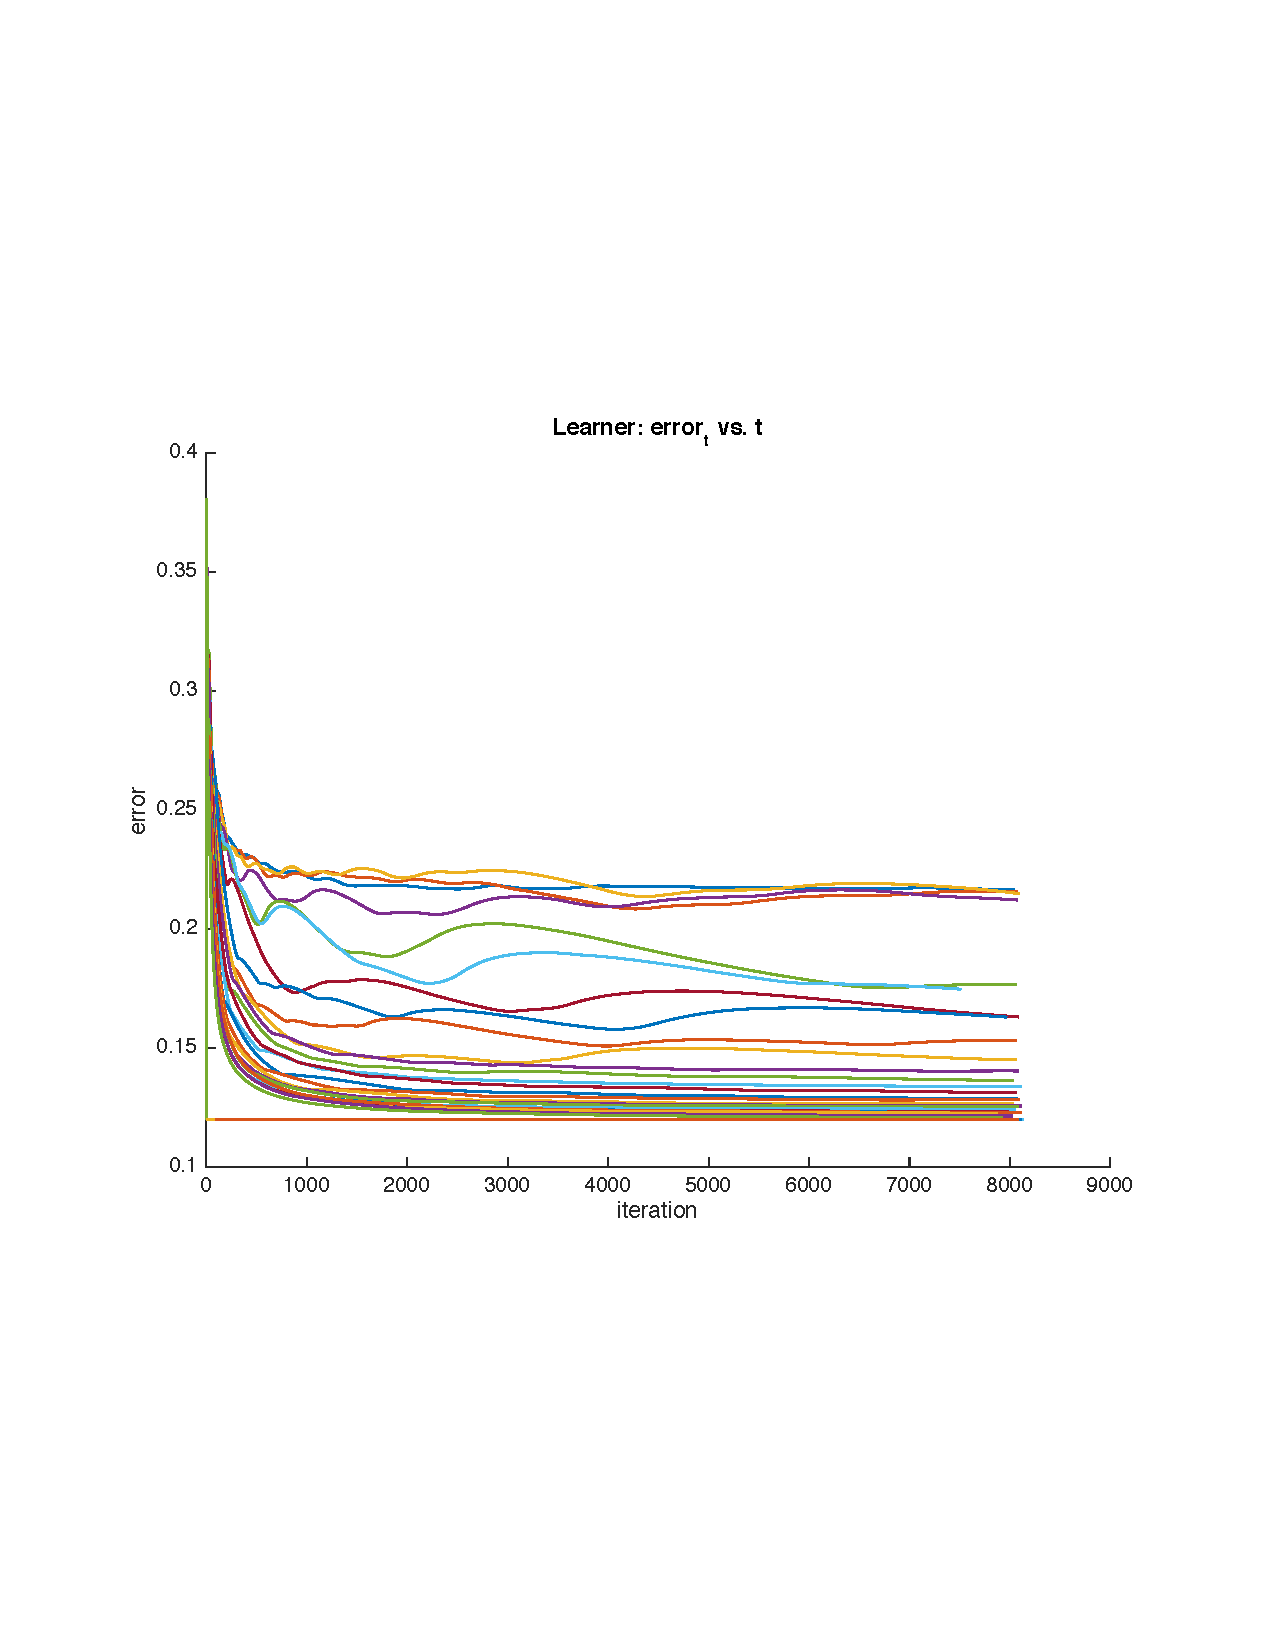
\includegraphics[scale=0.35]{nov20err.pdf}}
\subfigure[]{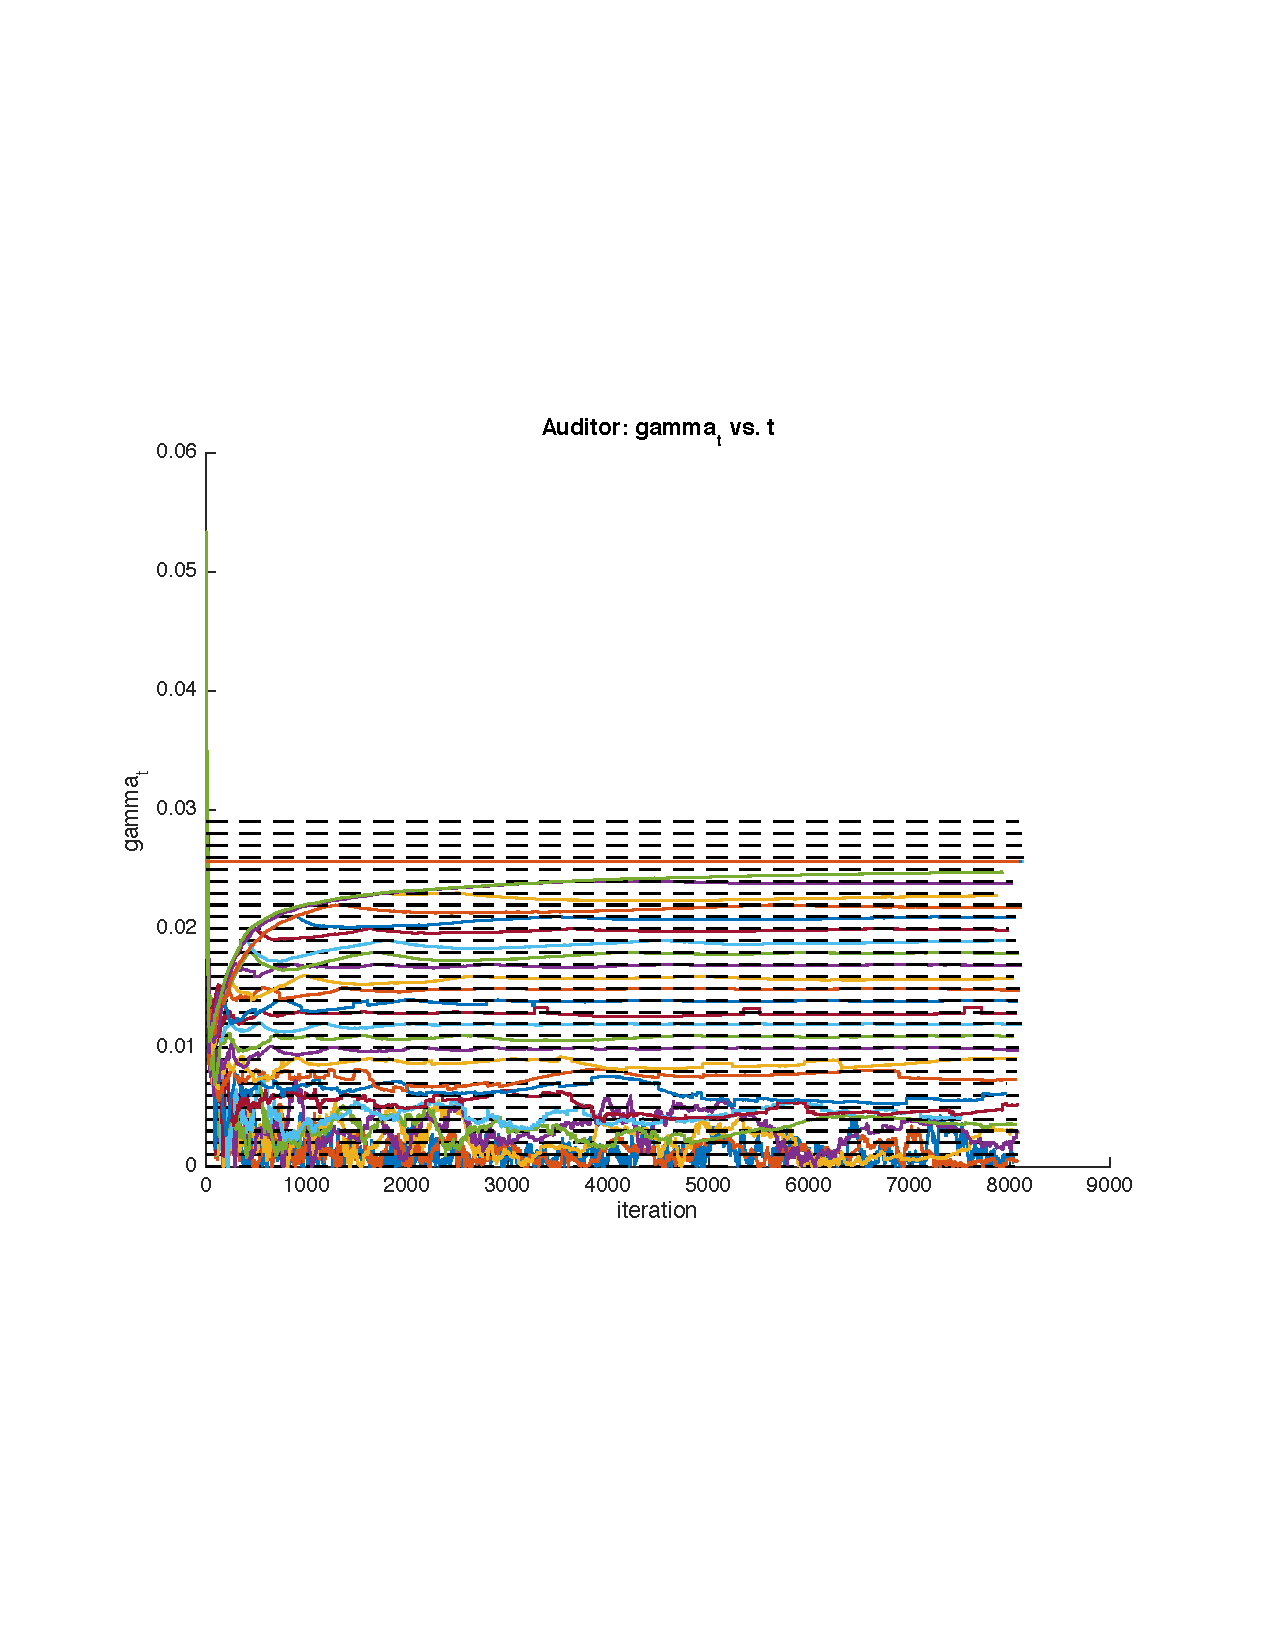
\includegraphics[scale=0.35]{nov20gamma.pdf}}
\caption{
Evolution of the error and unfairness of Learner's classifier across iterations,
for varying choices of $\gamma$.
(a) Error $\epsilon_t$ of Learner's model vs iteration $t$.
(b) Unfairness $\gamma_t$ of subgroup found by Auditor vs. iteration $t$, as measured
	by Definition~\ref{fp-fair}.
See text for details.
}
\label{fig:error}
\end{figure*}


We begin by examining the evolution of the error and unfairness of Learner's model.
In the left panel of Figure~\ref{fig:error} we show the error of the model found
by Learner vs. iteration for values of $\gamma$ ranging from 0 to 0.029.
Several comments are in order.

First, after an initial period in which there is a fair amount of oscillatory
behavior, by 6000 iterations most of the curves have largely flattened out,
and by 8,000 iterations it appears most but not all have reached approximate convergence.
Second, while the top-to-bottom ordering of these error curves is approximately
aligned with decreasing $\gamma$ --- so larger $\gamma$ generally results in lower error,
as expected --- there are many violations of this for small $t$, and even a few at large
$t$. Third, and as we will examine more closely shortly, the converged values
at large $t$ do indeed exhibit a range of errors.

In the right panel of Figure~\ref{fig:error}, we show the corresponding unfairness $\gamma_t$ of the subgroup
found by the Auditor at each iteration $t$ for the same runs and values of the parameter $\gamma$ (indicated by
horizontal dashed lines), with the same
color-coding as for the left panel. Now the ordering is generally reversed --- larger values of $\gamma$
generally lead to higher $\gamma_t$ curves, since the fairness constraint on the Learner is weaker.
We again see a great deal of early oscillatory behavior, with most $\gamma_t$ curves then eventually settling
at or near their corresponding input $\gamma$ value, as Learner and Auditor engage in a back-and-forth struggle
for lower error for Learner and $\gamma$-subgroup fairness for Auditor.

\begin{center}
\begin{figure*}[h]
\centering
\subfigure[]{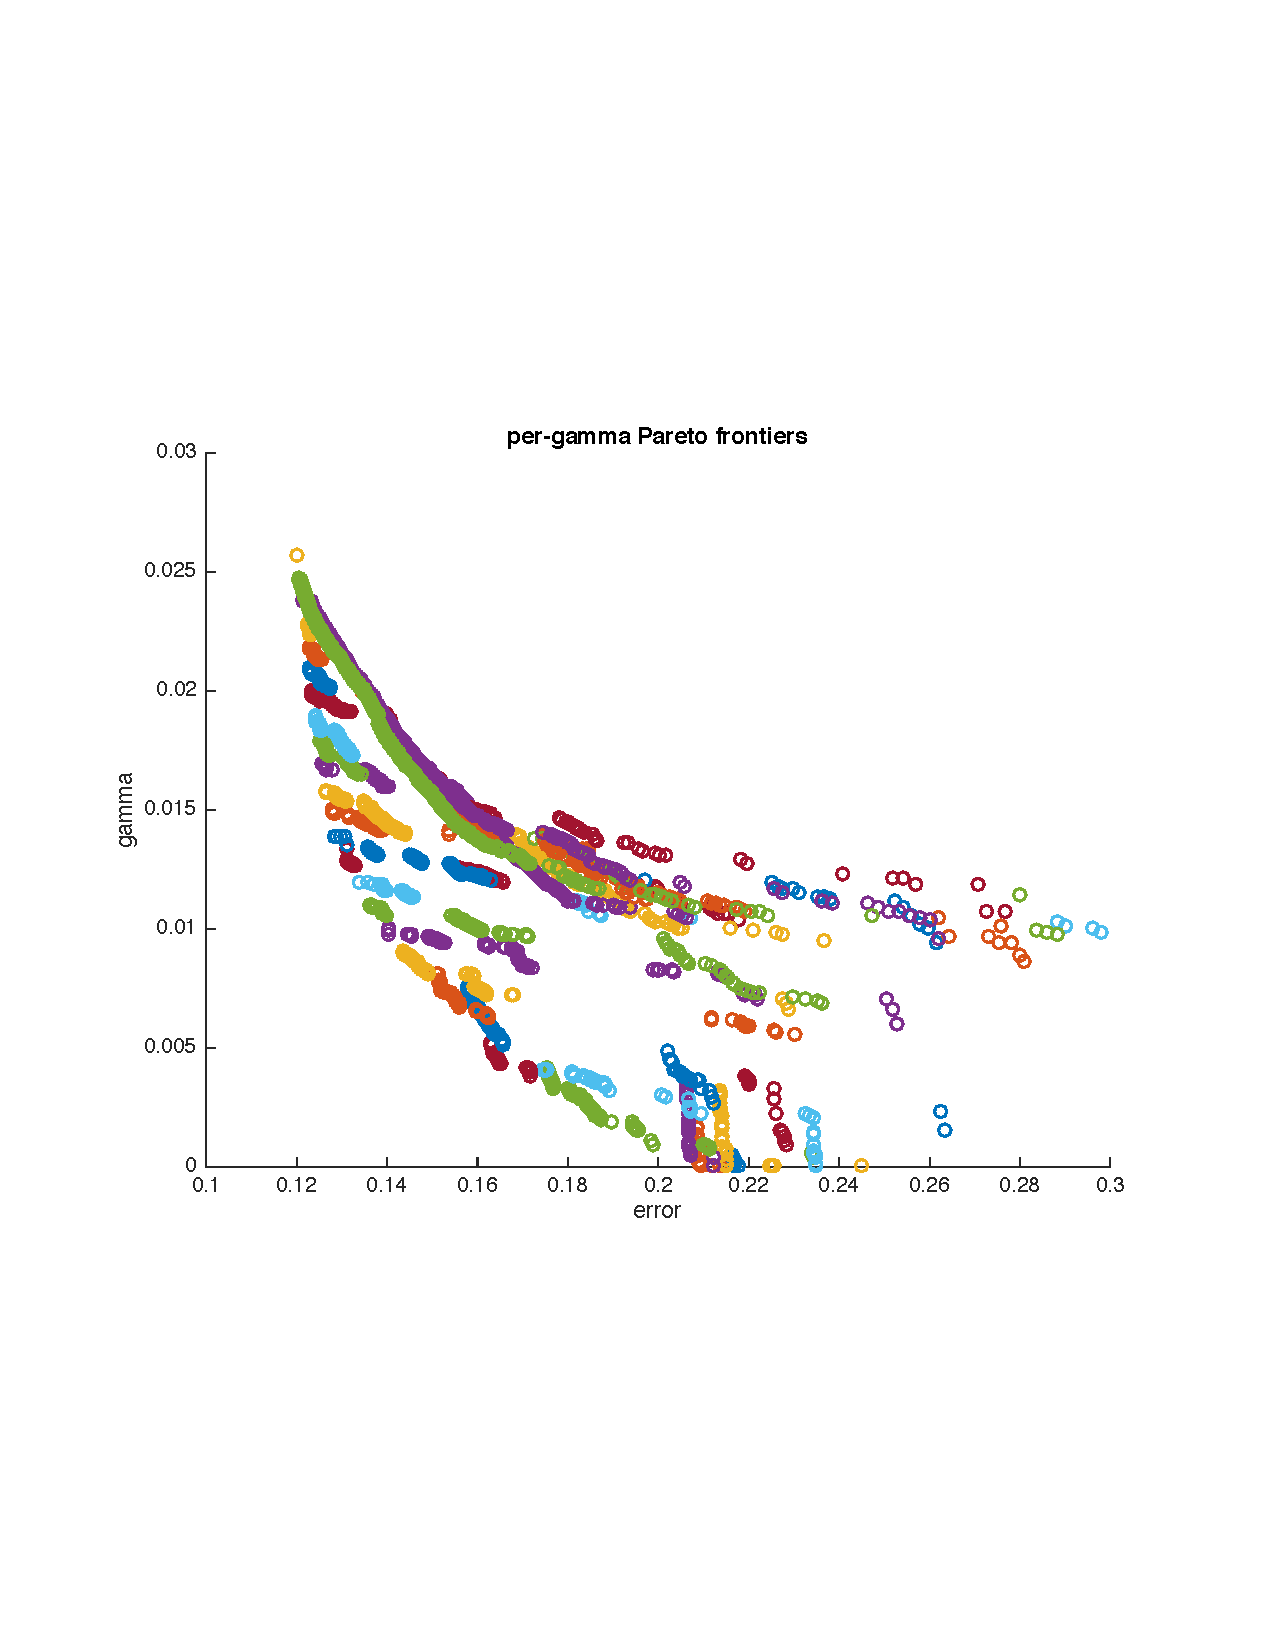
\includegraphics[scale=0.35]{nov20pergamma.pdf}}
\subfigure[]{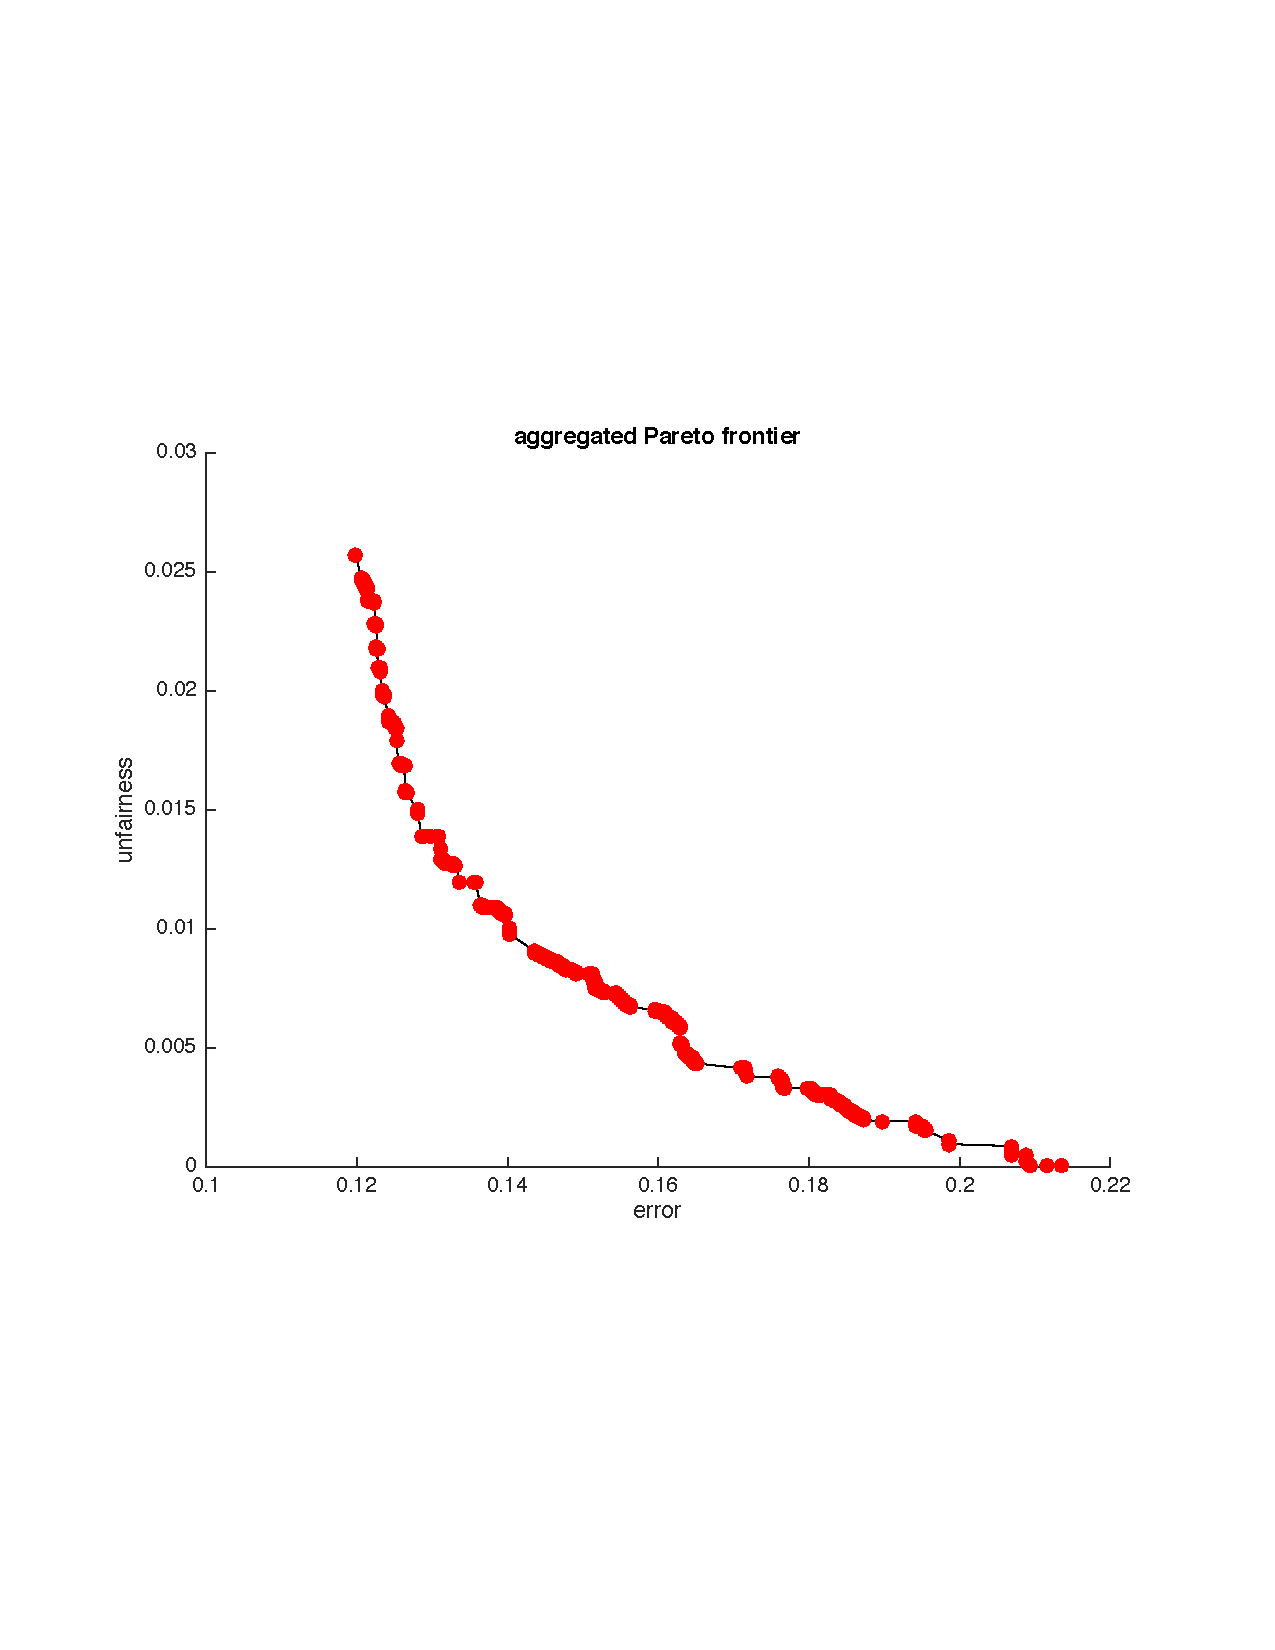
\includegraphics[scale=0.35]{nov20aggpareto.pdf}}
\caption{
(a) Pareto-optimal error-unfairness values, color coded by varying values of
	the input parameter $\gamma$.
(b) Aggregate Pareto frontier across all values of $\gamma$. Here the $\gamma$ values
cover the same range but are sampled more densely to get a smoother frontier.
See text for details.
}
\label{fig:fairness}
\end{figure*}
\end{center}

For any choice of the parameter $\gamma$, and each iteration $t$, the two panels of Figure~\ref{fig:error}
yield a pair of realized values $\langle \epsilon_t, \gamma_t \rangle$ from the experiment, corresponding to
a Learner model whose error is $\epsilon_t$, and for which the worst subgroup the Auditor was able to find
had unfairness $\gamma_t$.
The set of all
$\langle \epsilon_t, \gamma_t \rangle$
pairs across all runs or $\gamma$ values thus represents the
different trade-offs between error and unfairness found by our algorithm on the data.
Most of these pairs are of course Pareto-dominated by other pairs, so we are primarily
interested in the undominated frontier.

In the left panel of Figure~\ref{fig:fairness}, for each value of $\gamma$ we show the
Pareto-optimal pairs, color-coded for the value of $\gamma$. Each value of $\gamma$
yields a set or cloud of undominated pairs that are usually fairly close to each other, and
as expected, as $\gamma$ is increased, these clouds generally move leftwards and upwards
(lower error and higher unfairness).

We anticipate that the practical use of our algorithm would, as we have done,
explore many values of $\gamma$ and then pick a model corresponding to a point
on the aggregated Pareto frontier across all $\gamma$, which represents the collection
of all undominated models and the overall error-unfairness trade-off.
This aggregate frontier is shown in the right panel of
Figure~\ref{fig:fairness}, and shows a relatively smooth menu of options,
ranging from error about 0.21 and no unfairness at one extreme, to
error about 0.12 and unfairness 0.025 at the other, and an appealing
assortment of intermediate trade-offs. Of course, in a real application
the selection of a particular point on the frontier should be made in
a domain-specific manner by the stakeholders or policymakers in question.

\iffalse
While the analysis so far confirms that the Auditor indeed is enforcing fairness
constraints on the Learner, it does not provide a sense of the extent to which the
Auditor is finding multiple ``different'' subgroups over time, and is thus truly utilizing
the power of its rich space of models over the restricted attributes (in contrast to the more
traditional approach of ensuring fairness with respect to just one or a few pre-defined
protected groups). Perhaps the most basic way of measuring the diversity of subgroups found
by Auditor is to look at the actual evolution of the subgroup models --- in this case, the
weight vectors of the linear classifiers found. In Figure~\ref{fig:fairness}(b), we show
these weights over time for just the choice $C = 105$ (plots for other values of $C$ are
similar), and from iteration 10 to 1000 since the earliest weights are large and would dominate the
scale. It is clear from this figure that the Auditor indeed explores a diverse set of linear
classifiers over time, as many of the 18 protected attribute weights change sign repeatedly, a few
in sometimes oscillatory fashion.
But a more intuitive measure would be to simply look at how many datapoints are ``touched'' by the
Auditor over time --- that is, how many datapoints have fallen in one or more of the subgroups found
by the Auditor so far, which we can view as measuring the number of ``protected'' datapoints.
As the Auditor gradually finds more, and more diverse, subgroups to add to the Lagrangian of the
Learner, this quantity should increase. We illustrate this phenomenon in Figure~\ref{fig:fairness}(c),
which shows the cumulative number of datapoints touched by Auditor at each iteration, again for the
same selection of values of $C$. For all $C$ the $y$ value starts at 213, since the very first linear
classifier found by the Auditor defines a subgroup of 213 datapoints. For the smallest value of
$C$ ($C = 15$), the value eventually climbs to roughly half the dataset, while for the larger values of
$C$ the entire dataset is eventually touched by the Auditor. Note that this does not indicate that
fairness is obtained for every datapoint or subgroup, just that the Auditor has presented Learner
with fairness constraints involving every datapoint. Note that these values are reached very early
in the process (the first 30 iterations), despite the fact that the other plots clearly indicate that
the balance between accuracy and fairness continues long after.

\begin{center}
\begin{figure*}[h]
\subfigure[]{\includegraphics[scale=0.2]{pareto-fairness.jpg}}
\subfigure[]{\includegraphics[scale=0.2]{pareto-protected.jpg}}
% \subfigure[]{\includegraphics[scale=0.13]{pareto-lagrangian.jpg}}
\caption{
Pareto frontiers explored by varying $C$ across a wide range.
(a) Learner's error vs. subgroup unfairness.
(b) Learner's error vs. number of protected data points.
% (c) Learner's error vs. value of Lagrangian.
See text for details.
}
\label{fig:pareto}
\end{figure*}
\end{center}

We also illustrate the full spectrum of error-fairness trade-offs
yielded by running \FFP with values of $C$ ranging from 0 to 500. In
Figure~\ref{fig:pareto}(a), each point represents both the error ($x$ axis) and the
subgroup unfairness $u(g_T)$ at $T = 7000$ for varying values of $C$. While not all
points lie exactly on the Pareto frontier due to the differences in convergence rates,
a clear menu of near-optimal trade-offs emerges. We can have error near the unconstrained
optimal of 0.11, and subgroup unfairness over 0.06. At the other extreme, we can have
error no better than the trivial baseline of the constant classifier of 0.3, and near-zero
subgroup unfairness. In between there is an appealing curve of trade-offs, but one that
also cannot be escaped without enriching the model space of the Learner or the Auditor
or both. Figure~\ref{fig:pareto}(b) shows a similar frontier, this time between error
and the number of datapoints touched by Auditor as discussed above. Again we see a menu
of trade-off options, from optimal error and few subgroup members, to progressively worse
error and the entire population involved in audited subgroups.
\fi

\iffalse
From output of running python MSR_Reduction.py 18 'communities' 25 > msr.out
13
('fp_disparity in each group: [0.0013113716353717608, 0.0046625099984154428, 0.0056142003818107633, 0.0016257868345736504, 0.014275573709644052, 0.0088216680094329591, 0.00
072916236199982443, 0.0032984555896687917, 0.0013294130549362237, 0.0075408798320930059, 0.0099591201679069541, 0.00024781495513553908, 0.0066228212355226579, 0.00019045248
166565942, 0.022459120167907021, 0.0039107330711327659, 0.00035641381267559336, 0.0010305487393355572, 0.0010305487393355017, 0.0048915526003394105, 0.00025203569924209246,
 0.00081674190105857081, 0.0038120662727710308, 0.002626717933270073, 0.00051667412474148966, 0.012156264447477638, 0.016788191660050023, 0.0016257868345736504, 0.000729162
36199982443]',)
max fp disparity in each group: 0.0224591201679
error of h: 0.159979939819
the fp rate in the group is 0.690322580645
the fp base rate overall is: 0.427685950413
the weight of the subgroup is: 0.674022066199
the relative error increase is: 61.4087579866%
group membership: [1 1 1 ..., 0 1 1]
subgroup coefficients: [[ -4.79716798e+00  -5.38116487e+00   1.31801264e+01  -3.99783937e+00
    9.44021934e-02  -7.08771131e-01   2.52249752e-01  -1.27488175e-01
    3.72468103e-02   5.72108311e+01   1.60989037e+00  -3.22004317e+00
   -9.14819945e-01   2.07579453e+00   1.86595122e+02   1.58550270e+02
   -2.31421903e+01  -2.93555046e+02]]
closest conjunction: [[ 1.  1. -1.  1. -1.  1. -1.  1. -1. -1. -1.  1.  1. -1. -1. -1.  1.  1.]]*x < [ 7.]
the group attributes are: ['racePctWhite', 'racePctAsian', 'racePctHisp', 'agePct12t21', 'blackPerCap', 'indianPerCap', 'AsianPerCap', 'OtherPerCap', 'HispPerCap', 'NumUnde
rPov', 'PctNotSpeakEnglWell', 'PctLargHouseFam', 'PctBornSameState', 'PctPolicWhite', 'PctPolicBlack', 'PctPolicHisp', 'PctPolicAsian', 'PctPolicMinor']
14


\subsection{Protecting Marginal Subgroups is not Sufficient}

It is intuitive that one can construct (as we did in the introduction)
artificial examples in which classifiers which equalize false positive rates across groups defined only with respect to individual protected binary features can exhibit unfairness in more complicated subgroups.
However, it might be the case that on real-world datasets, enforcing false positive rate fairness
only in marginal subgroups, using
previously known algorithms (like  \cite{reductions}), would already provide at least approximate fairness
in the combinatorially many subgroups defined by a simple (e.g. linear threshold) function over the protected features.
In this case our more elaborate techniques and guarantees would not be needed except for in theory.

To explore this possibility,
we implemented the algorithm of \cite{reductions}, which employs a
similar optimization framework. In their algorithm the primal player
plays the same weighted classification oracle we use, and the dual
player plays gradient descent over a space of dimension equal to the number of protected groups.
We used the same Communities and Crime dataset with the same $18$ protected features.
Our 18 protected attributes are real valued. In order to come up with a
small number of protected groups, we threshold each real-valued
attribute at its mean, and define 36 protected groups: each one corresponding
to one of the protected attributes lying either above or below its mean.
% we thresholded the violent crime variable at the 20th percentile, creating a dataset
% with a higher base rate which is consequently harder to enforce False Positive fairness on.

We then ran the algorithm from  \cite{reductions}.
The algorithm converges to a lowest achieved marginal false positive 
rate of

However, upon auditing the resulting classifier with respect to the richer
class of linear threshold functions on the continuously-valued
protected features, we discover a large subgroup whose false positive
rate differed substantially from the baseline. This subgroup had
weight $0.674$ (consisting of well over half of the datapoints),
and a false positive rate that was higher than the base rate by $0.26$ --- a 61\% increase.
While the discriminated subgroup is of course defined by a complex linear threshold function over 18 variables,
the largest weights by far were on only three of these features, and the subgroup can thus be informally
interpreted as a disjunction identifying communities where the percentage of the police forces
that are Black or Hispanic are relatively high, or where the percentage that is Asian is relatively low.

This simple experiment illustrates that in practice it may be easy
to learn classifiers which appear fair with respect to the
marginal groups given by pre-defined protected features, but may
discriminate significantly against the members of a simple combinatorial subgroup.
We suspect this phenomenon is common on many datasets, and that our methods and algorithms are needed
to address it.
\fi
